\section{Analysis}\label{sec:analysis}

    \subsection{Data and noise}\label{sec:data}
        The function, onto which we are trying to fit a model, is the Franke Function(cite this). It is defined as follows:
        \begin{align}\label{eq:francefunc}
            f(x,y) &= \frac{3}{4}\exp{-\frac{(9x-2)^2}{4}-\frac{(9y-2)^2}{4}} \nonumber\\
            &+ \frac{3}{4}\exp{-\frac{(9x+1)^2}{49}-\frac{(9y+1)}{10}} \nonumber\\
            &+ \frac{1}{2}\exp{-\frac{(9x-7)^2}{4}-\frac{(9y-3)^2}{4}} \nonumber\\
            &-\frac{1}{5}\exp{-(9x-4)^2-(9y-7)^2}.
        \end{align}
        In order to generate a dataset we will use $N$ uniformly distributed values of $x,y\in[0,1]$. We will also add some normally distributed noise $\epsilon = \eta\mathcal{N}(\mu,\sigma^2) = \eta\mathcal{N}(0,1)$ to $f(x,y)$, where $\eta$ is a strength parameter controlling the amplitude of the added noise. The full description of our data then become:
        \begin{align}\label{eq:datadescription}
            \vec{y} &= f(x,y) + \eta\mathcal{N}(0,1) \nonumber \\
            &= f(\vec{x}) + \epsilon
        \end{align}
        where $\vec{x} = (x,y)$. 
        NECESSARY?From section \Sec{regression} we have a model for this data: $\tilde{\vec{y}} = X\hat{\svec{\beta}}$ where $X$ is the design matrix and $\hat{\svec{\beta}}$ are the optimal parameters which we are trying to determine. 

        We visualise the data both with and without noise. Figure \Fig{franke_function} shows the Franke function without any noise ($\eta=0$), plotted for uniformly distributed $x$ and $y$, where $N=40$. Figure \Fig{franke_function_noise} show the same function, for the same points but now with an added noise of $\eta=0.1$.

        \begin{figure}
            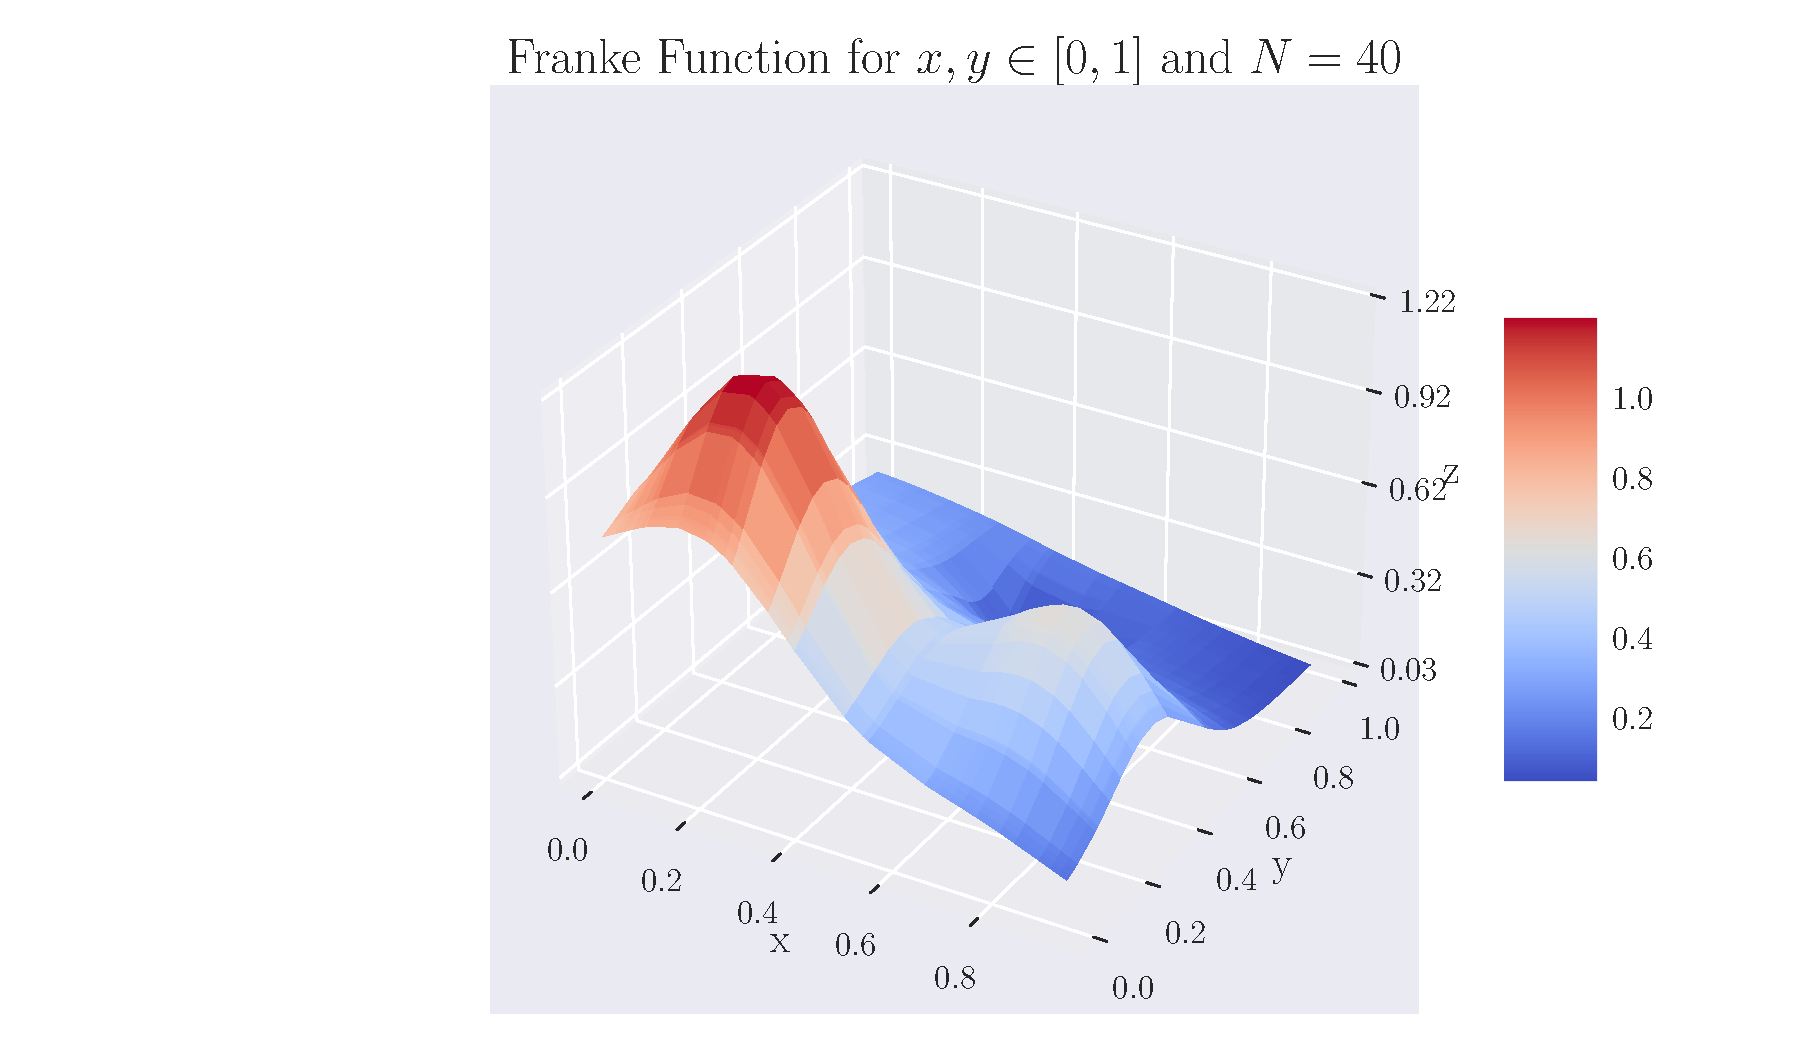
\includegraphics[width=\linewidth]{franke.pdf}
            \caption{The Franke function plotted on a grid where $N=40$ and $\eta=0$}
            \label{fig:franke_function}
        \end{figure}

        \begin{figure}
            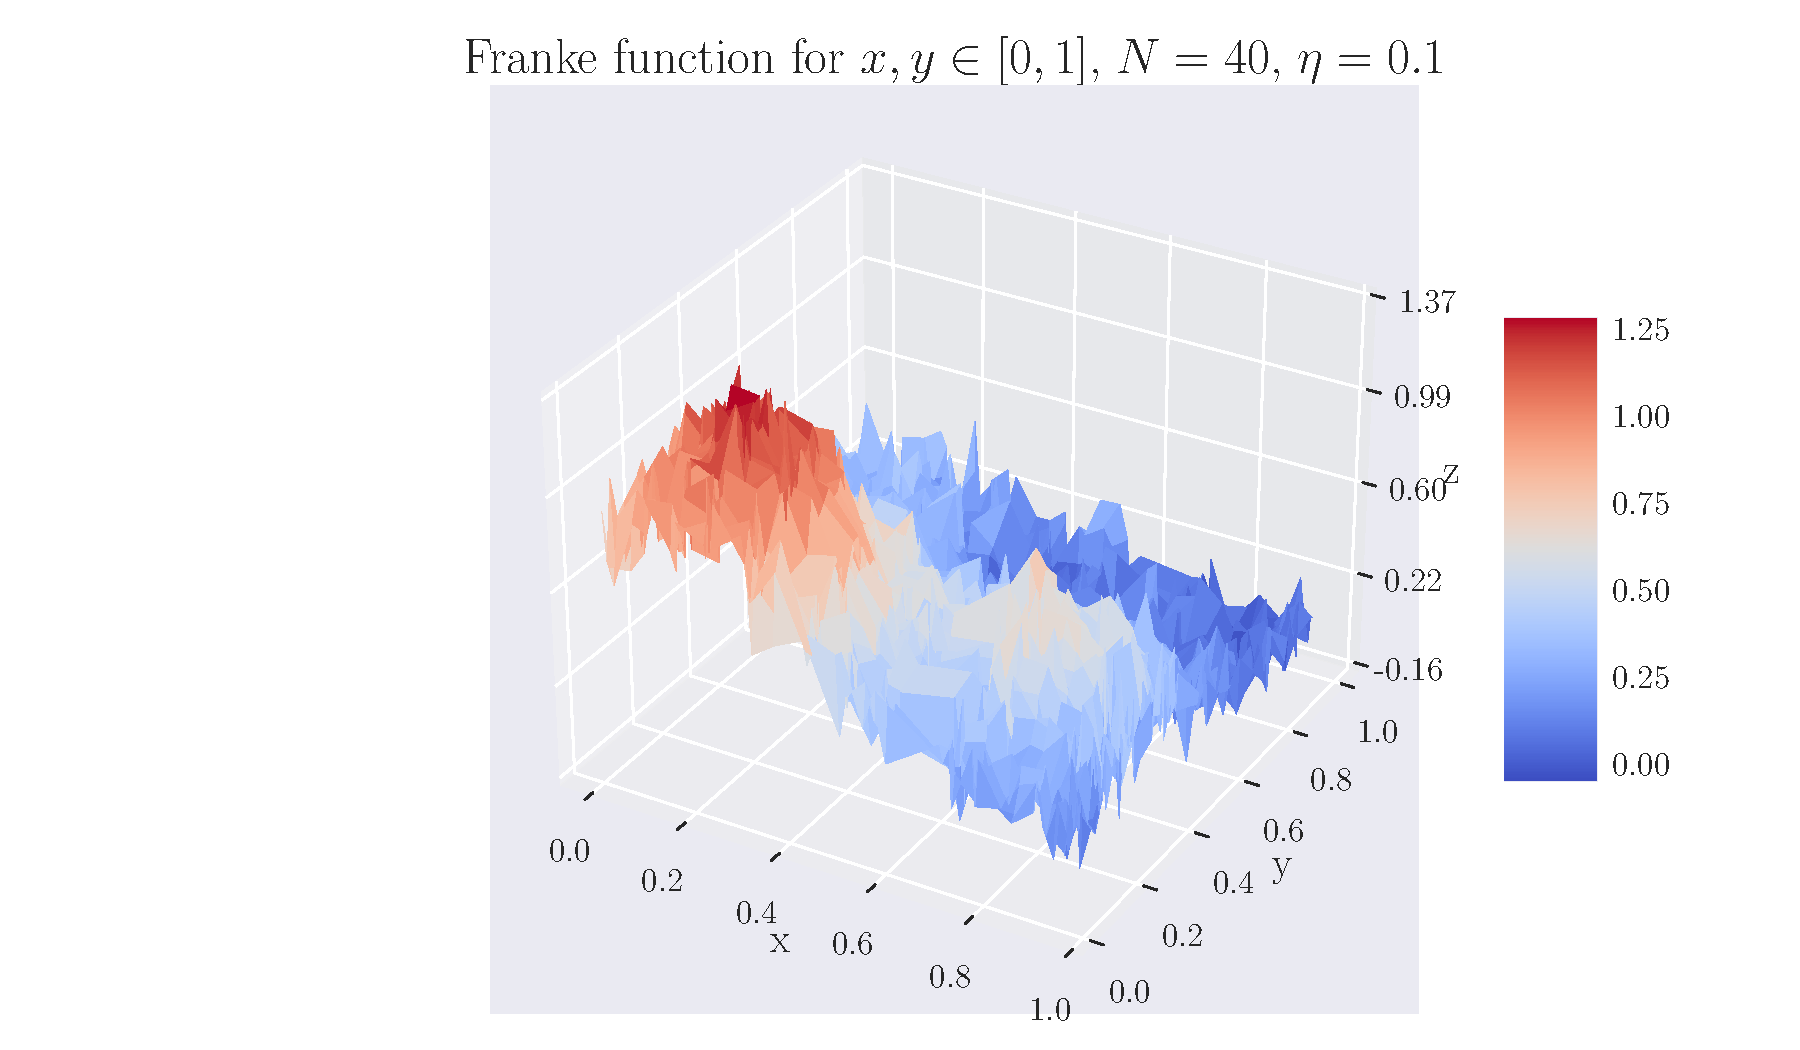
\includegraphics[width=\linewidth]{franke_noise.pdf}
            \caption{The Franke function with added noise plotted on a grid where $N=40$ and $\eta=0.1$}
            \label{fig:franke_function_noise}
        \end{figure}

    \subsection{Data splitting}\label{sec:splitting}
        In order to test our estimate of $\hat{\svec{\beta}}$ we reserve some of the data for testing. We thus divide our data set into a part for testing a part for training. We select 80 \% of the data for training and the remaining 20 \% for testing the data. The data is split at random. 

    \subsection{Model and design matrix}\label{sec:model}
        The design matrix $X$ has dimensionality ($n\cross p$) where $n$ represents the data points and $p$ the features of the model. We have already split the data set into training and testing, and must therefore create two design matrices: $X_{\text{train}}$ and $X_{\text{test}}$. 
        \\
        We want our model to be a two-dimensional polynomial of order $d$:
        \begin{align*}
            P_d(x,y) = \beta_0 + \sum_{l=1}^d\sum_{k=0}^{l} \beta_jx^{l-k}y^k
        \end{align*}
        where $j\in[1,p]$ and $p=(d+1)\cdot\left[(d+2)/2\right]$ is the number of features, or number of terms in a two dimensional polynomial. $\beta_0$ is our intercept (constant term). From this we set up the design matrix with the following terms (THIS IS WRONG; CORRECT THIS):
        \begin{align}\label{eq:designmatrixequation}
            X_{ij} = \sum_{l=1}^d\sum_{k=0}^{l} x^{l-k}y^k
        \end{align}
        The design matrix is set up without an intercept (constant term) (WHY?). Since we need to set up to design matrices, they account for a different amount of data points, and thus $n$ will be different between the two, but $p$ is the same. 
    \subsection{Scaling}\label{sec:scaling}
        We want to scale both our data and the design matrices because the data obtained from either the Franke function, or from some other source often vary a great deal in magnitude. Since the design matrices are set up in order to fit data to a polynomial of degree $d$ in two dimensions, we want to be sure that no term is given more emphasis than the others. In addition, when working with multi-dimensional data and design matrices we want to standardize the features as much as possible to ensure equal (relative) emphasize and treatment of the dimensions. We use the scaling technique \textit{standardization} or \textit{Z-score normalization} which makes the mean of each feature equal to zero, and the their variances to be of unit length. For our observed data $\vec{y}$ this mean:
        \begin{align*}
            \vec{y}' = \frac{\vec{y}-\bar{\vec{y}}}{\sigma_{\vec{y}}}
        \end{align*}
        where $\vec{y}'$ is now our scaled data. For the design matrices, this must be done for each feature, i.e. for each column.  Mathematically, if $X_j$ is column $j$ of the original design matrix $X$, $j\in[0,p]$:
        \begin{align*}
            X_j' = \frac{X_j-\bar{X_j}}{\sigma_{X_j}}.
        \end{align*}
        We do this for all the columns and end up with the scaled design matrix $X'$. Since $\optbeta$ is a function of the design matrix $X$ and the data $\vec{y}$,
        
        MORE ON WHY EVERYTHING NEED TO BE SCALED WRT TRAIN Data

    \begin{align*}
        \optbeta' = \optbeta\frac{\sigma_X}{\sigma_{\vec{y}}} \implies \optbeta = \optbeta'\frac{\sigma_{\vec{y}}}{\sigma_X}
    \end{align*}


    \subsection{Regression analysis}\label{sec:reganalysis}

        \subsubsection{OLS}\label{sec:olsanalysis}
            We start by performing an Ordinary Least Square regression analysis, as outlined in section \Sec{OLS}, where we find $\hat{\svec{\beta}}^\text{OLS}$ from \Eq{optimal_beta_ols} and $\variance{\optbeta^{\text{OLS}}}$ from \Eq{variance_of_optimal_beta_ols}. The error can be estimated with the standard deviation $\vec{\sigma}_{\beta} = \variance{\optbeta^{\text{OLS}}}^{1/2}$. 

            We have scaled the data and removed the intercept, thus we do not concern ourselves with $\beta_0$, so $\svec{\beta}^{\text{OLS}} = (\beta_1, \beta_2, \beta_3, \dots, \beta_{p-1})$. We train models, i.e. we find $\optbeta^{\text{OLS}}$ for polynomials up to order $5$. The values of these optimal parameters are plotted in \Fig{beta_with_standard_deviation}, with error bars of one standard deviation. We notice that the variation of the feature parameters increase as the polynomial degree of the model increase. This is expected because when the complexity of the model increase, it want to traverse more points exactly. 

            \begin{figure}
                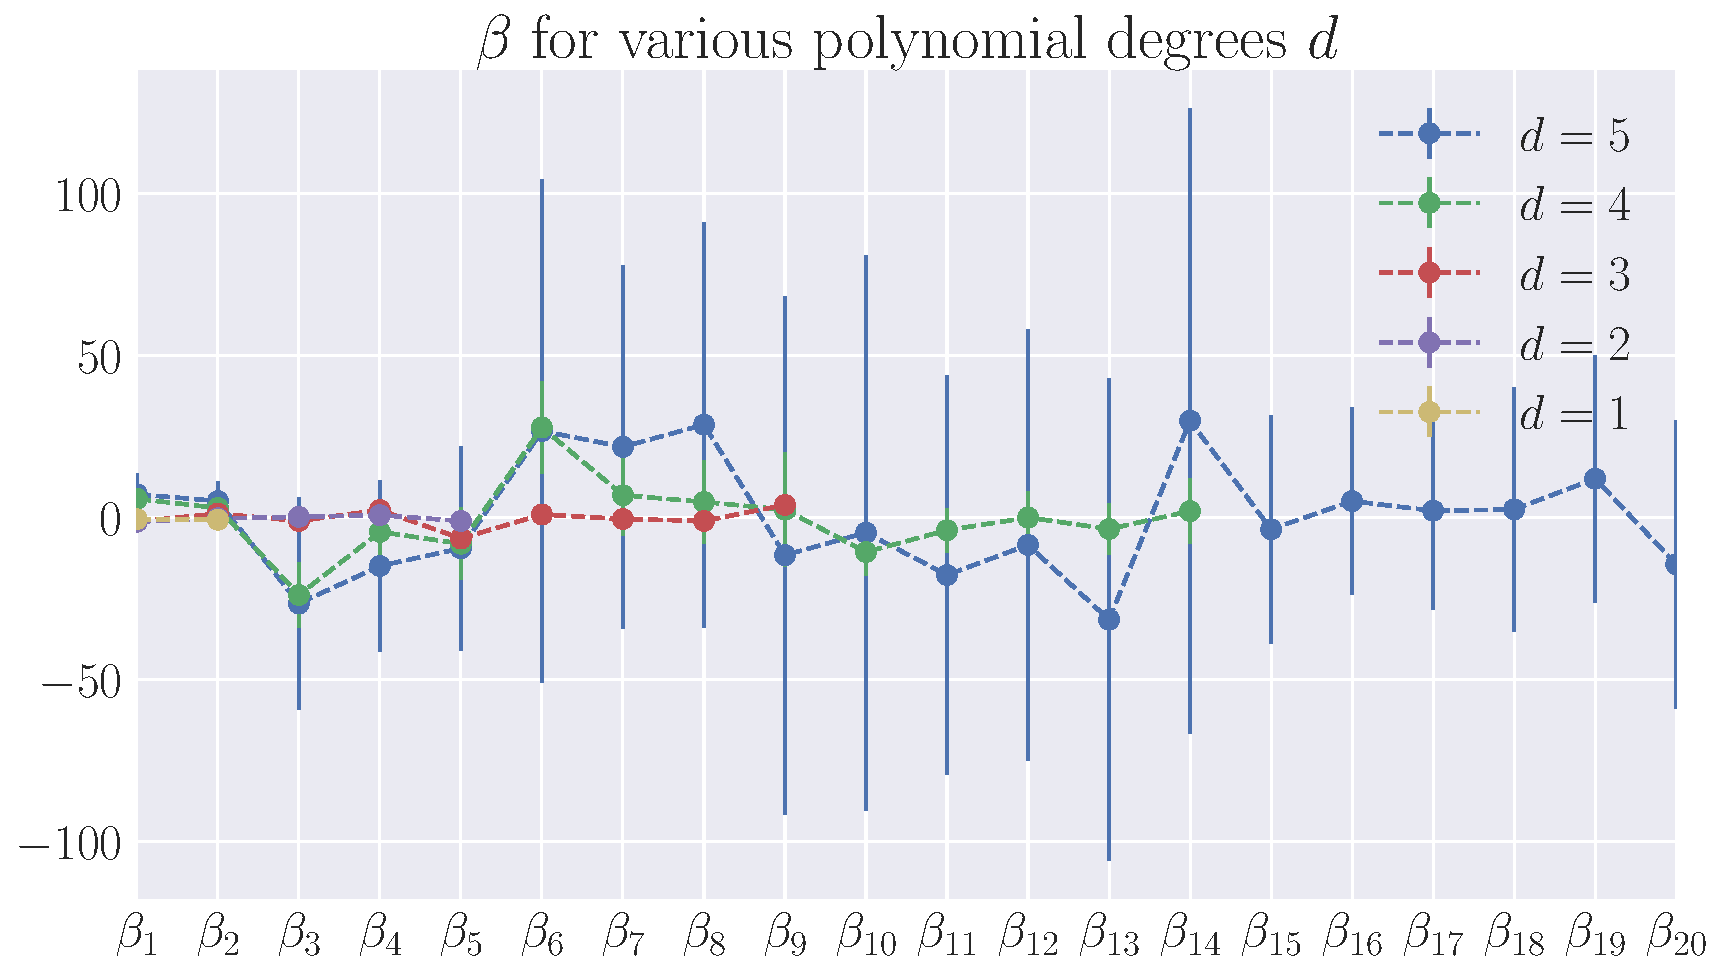
\includegraphics[width=\linewidth]{ptB_betas.pdf}
                \caption{Numerical value of the feature parameters $\beta$, with 1$\sigma$ error bars, for polynomials up to order $d=5$.}
                \label{fig:beta_with_standard_deviation}
            \end{figure}

            Having found the optimal parameter $\optbeta^{\text{OLS}}$ we can make predictions by computing $\tilde{\vec{y}} = X\optbeta^{\text{OLS}}$ for both the training data and the test data. In order to say something about the quality of these predictions we compute the mean square error and the $R^2$ score from equations \Eq{MSE} and \Eq{R2} respectively. The result of this is shown in \Fig{mse_and_r2_for_order5}. COMMENT ON PLOT
            \begin{figure}
                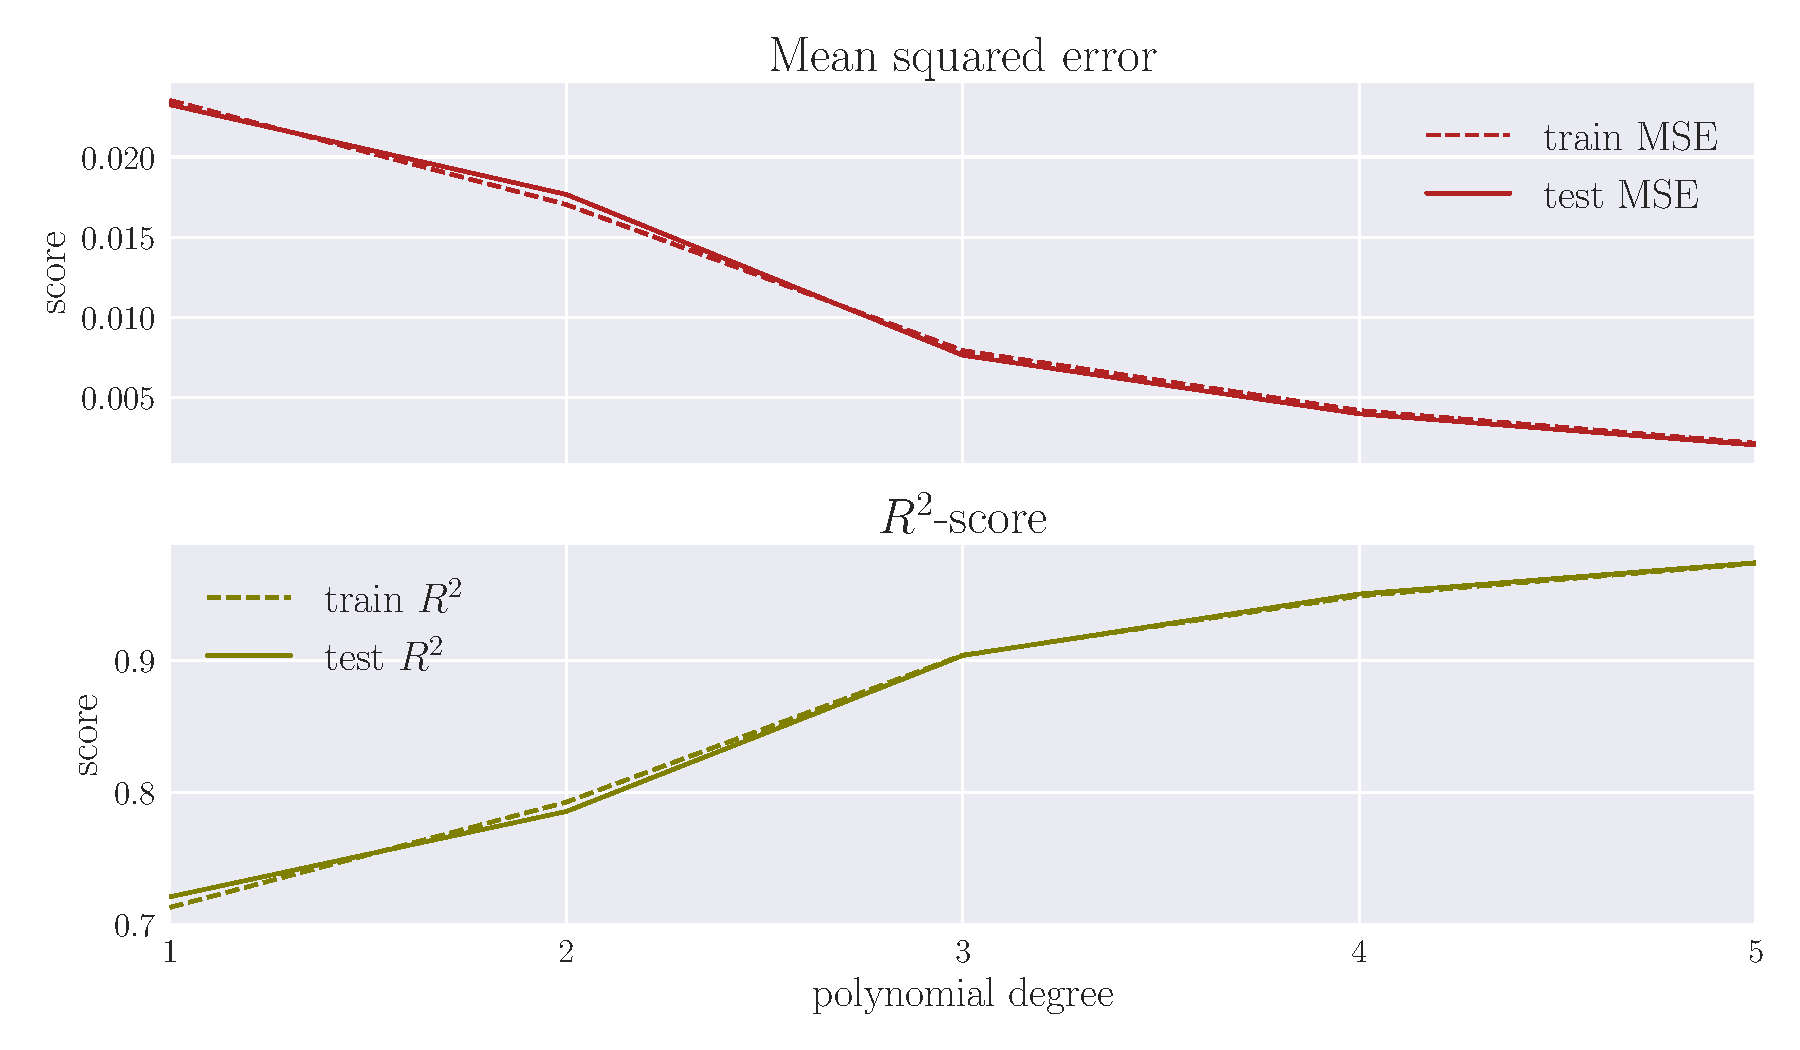
\includegraphics[width=\linewidth]{ptB_scores.pdf}
                \caption{SCORES}
                \label{fig:mse_and_r2_for_order5}
            \end{figure}

           

            \begin{figure}
                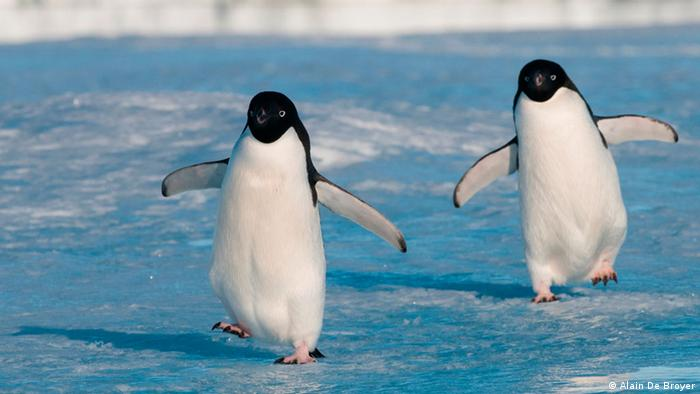
\includegraphics[width=\linewidth]{dummy.jpg}
                \caption{MSE error for different noise values $\eta$}
                \label{fig:mse_for_different_noise_ols}
            \end{figure}

            SOMETHING ABOUT NOSIE

            \begin{figure}
                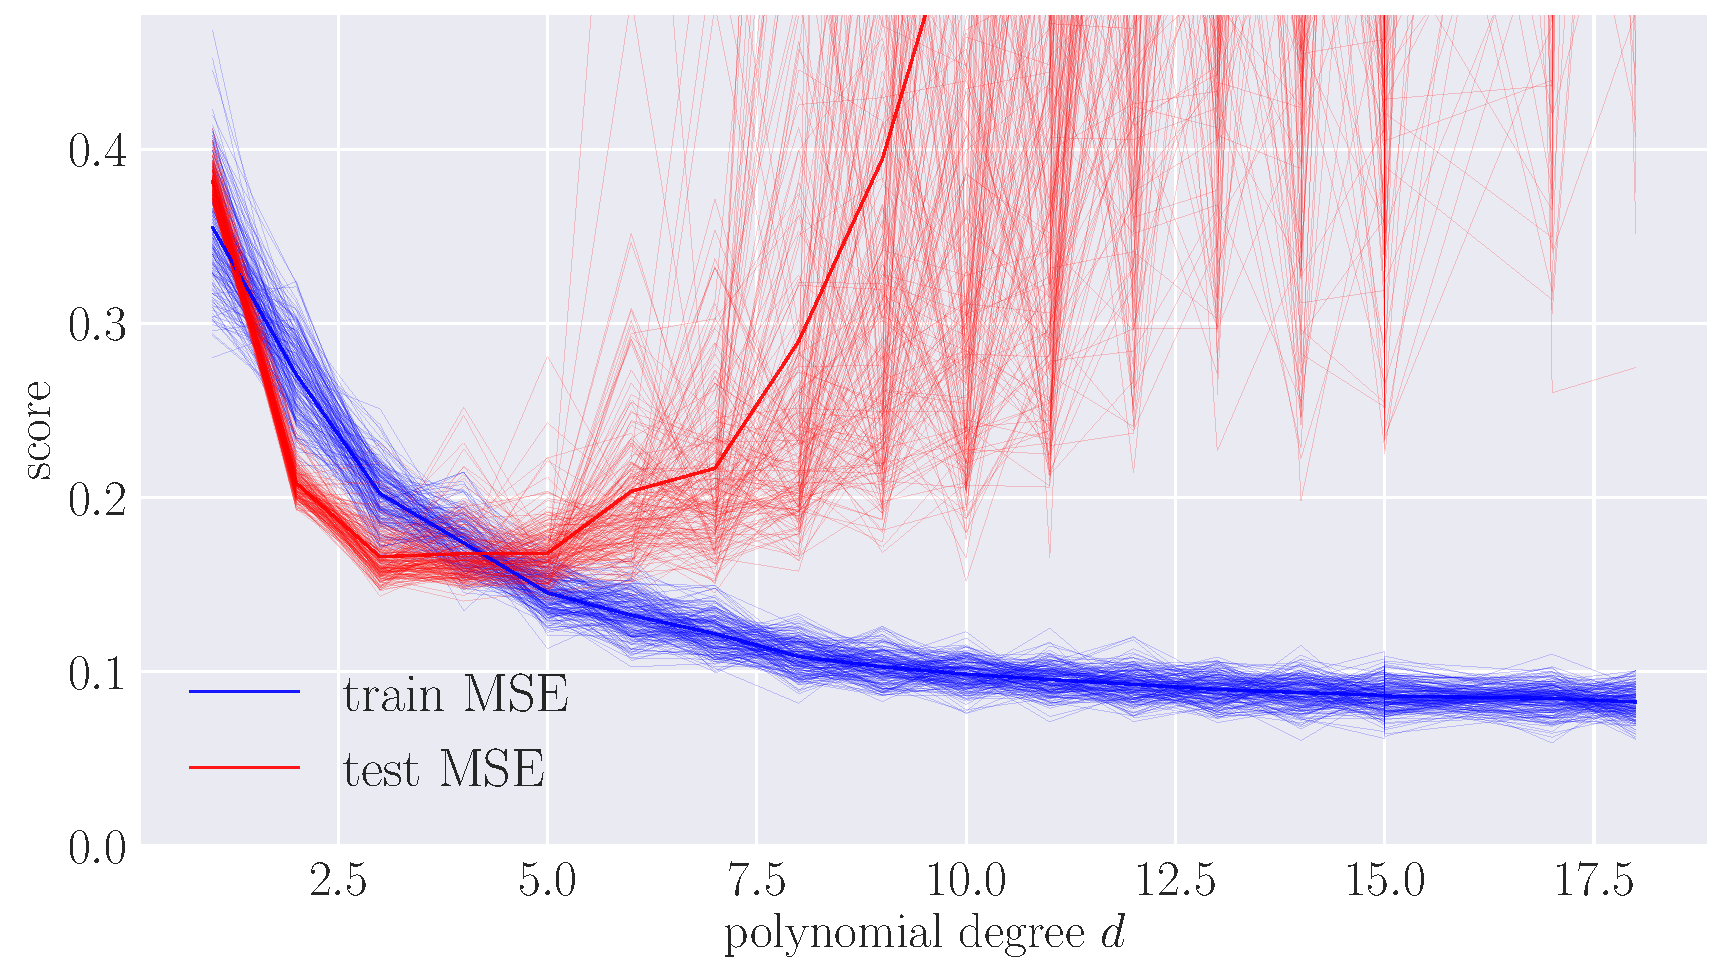
\includegraphics[width=\linewidth]{ptC_Hastie_OLS.pdf}
                \caption{Model complexity HASTIE ET AL.}
                \label{fig:model_complexity_ols}
            \end{figure}

            \begin{figure}
                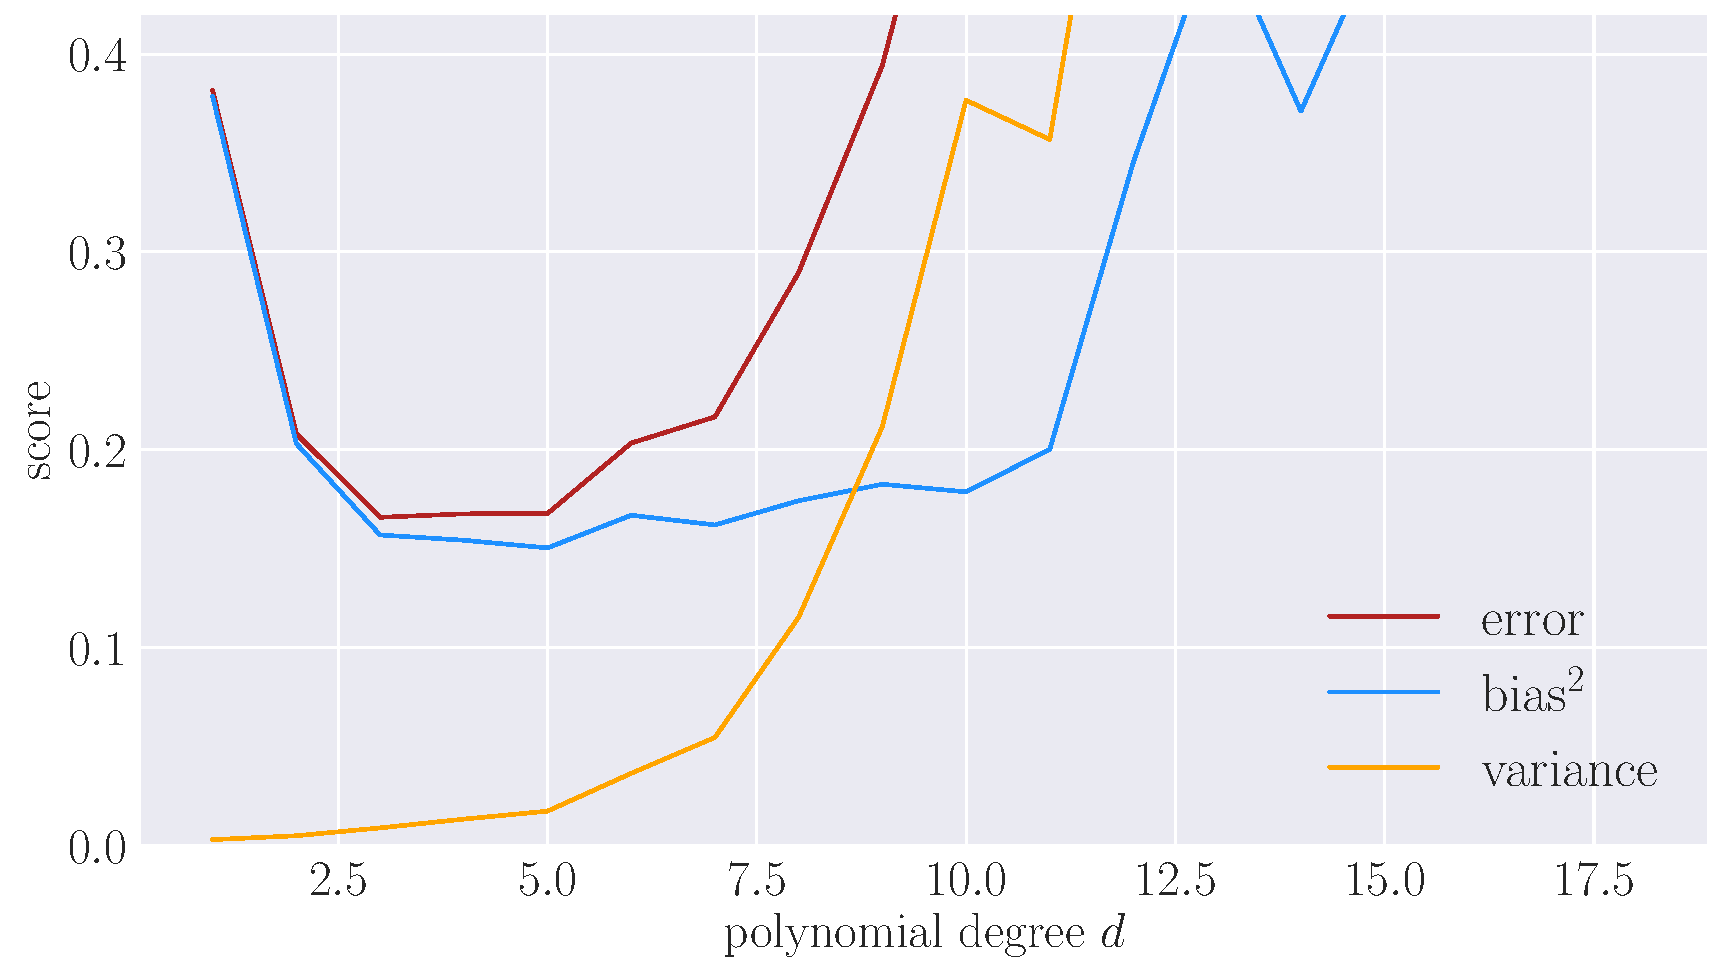
\includegraphics[width=\linewidth]{ptC_tradeoff_OLS.pdf}
                \caption{Bias Variance}
                \label{fig:bias_variance_ols}
            \end{figure}


            \begin{figure}
                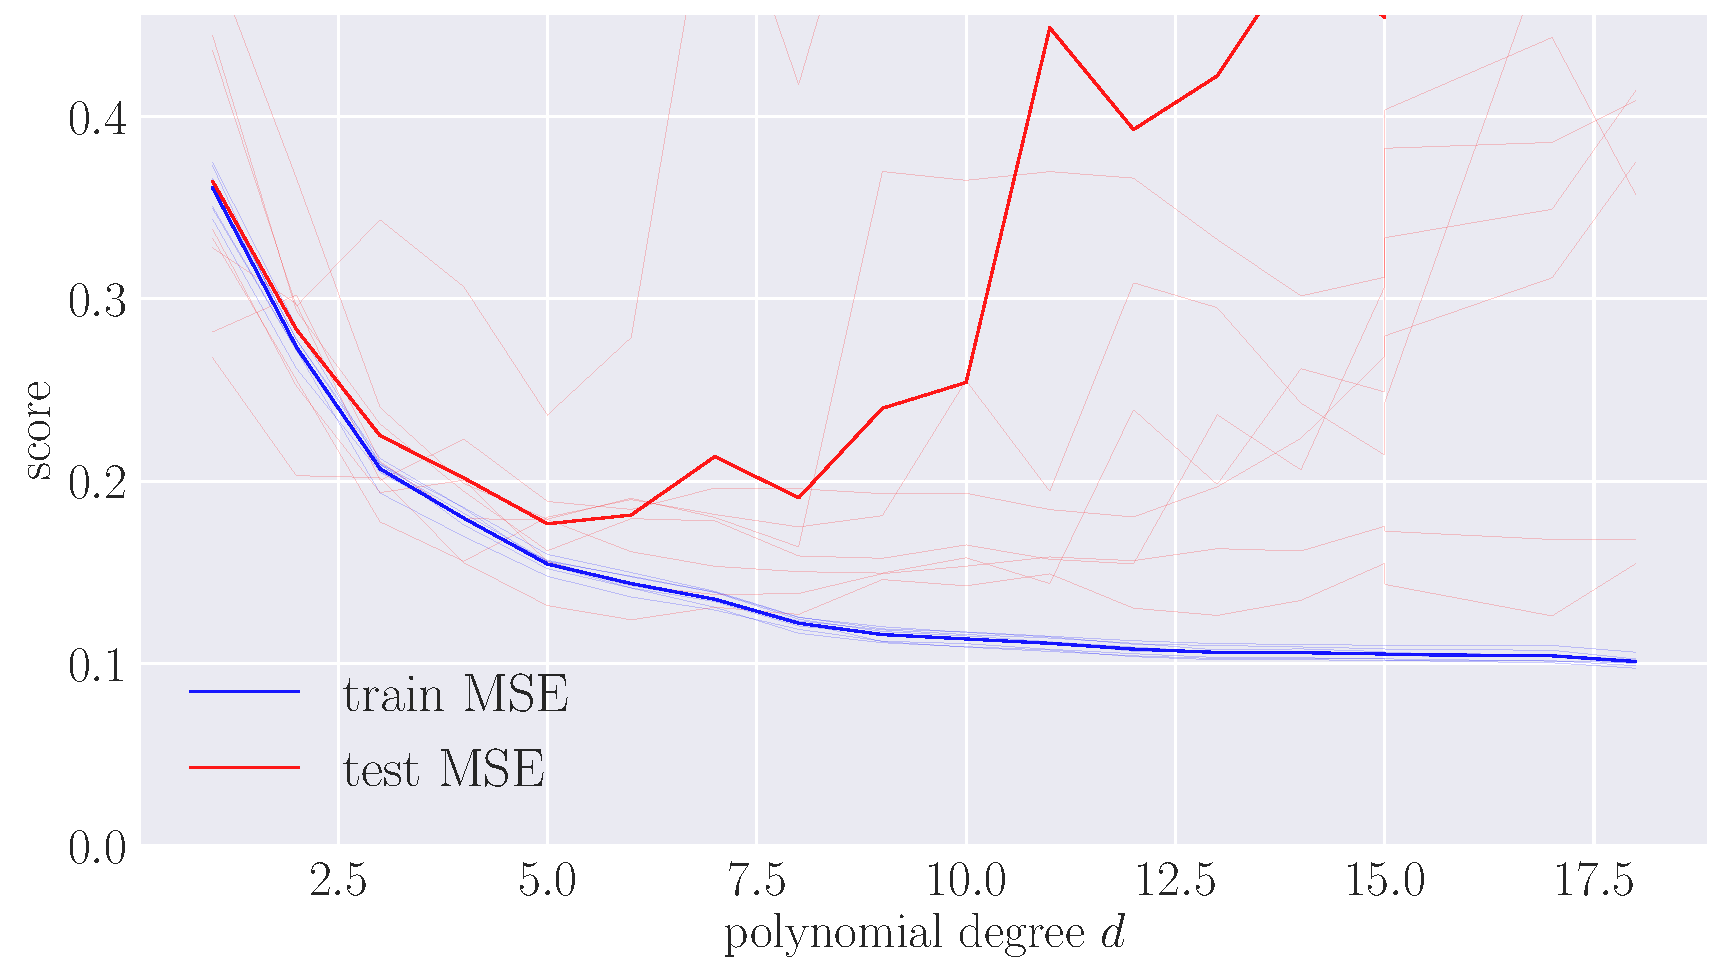
\includegraphics[width=\linewidth]{ptD_CV_OLS.pdf}
                \caption{Cross-validation}
                \label{fig:cross-validation_ols}
            \end{figure}



        

        \subsubsection{Ridge}\label{sec:rigdeanalysis}

        \begin{figure}
            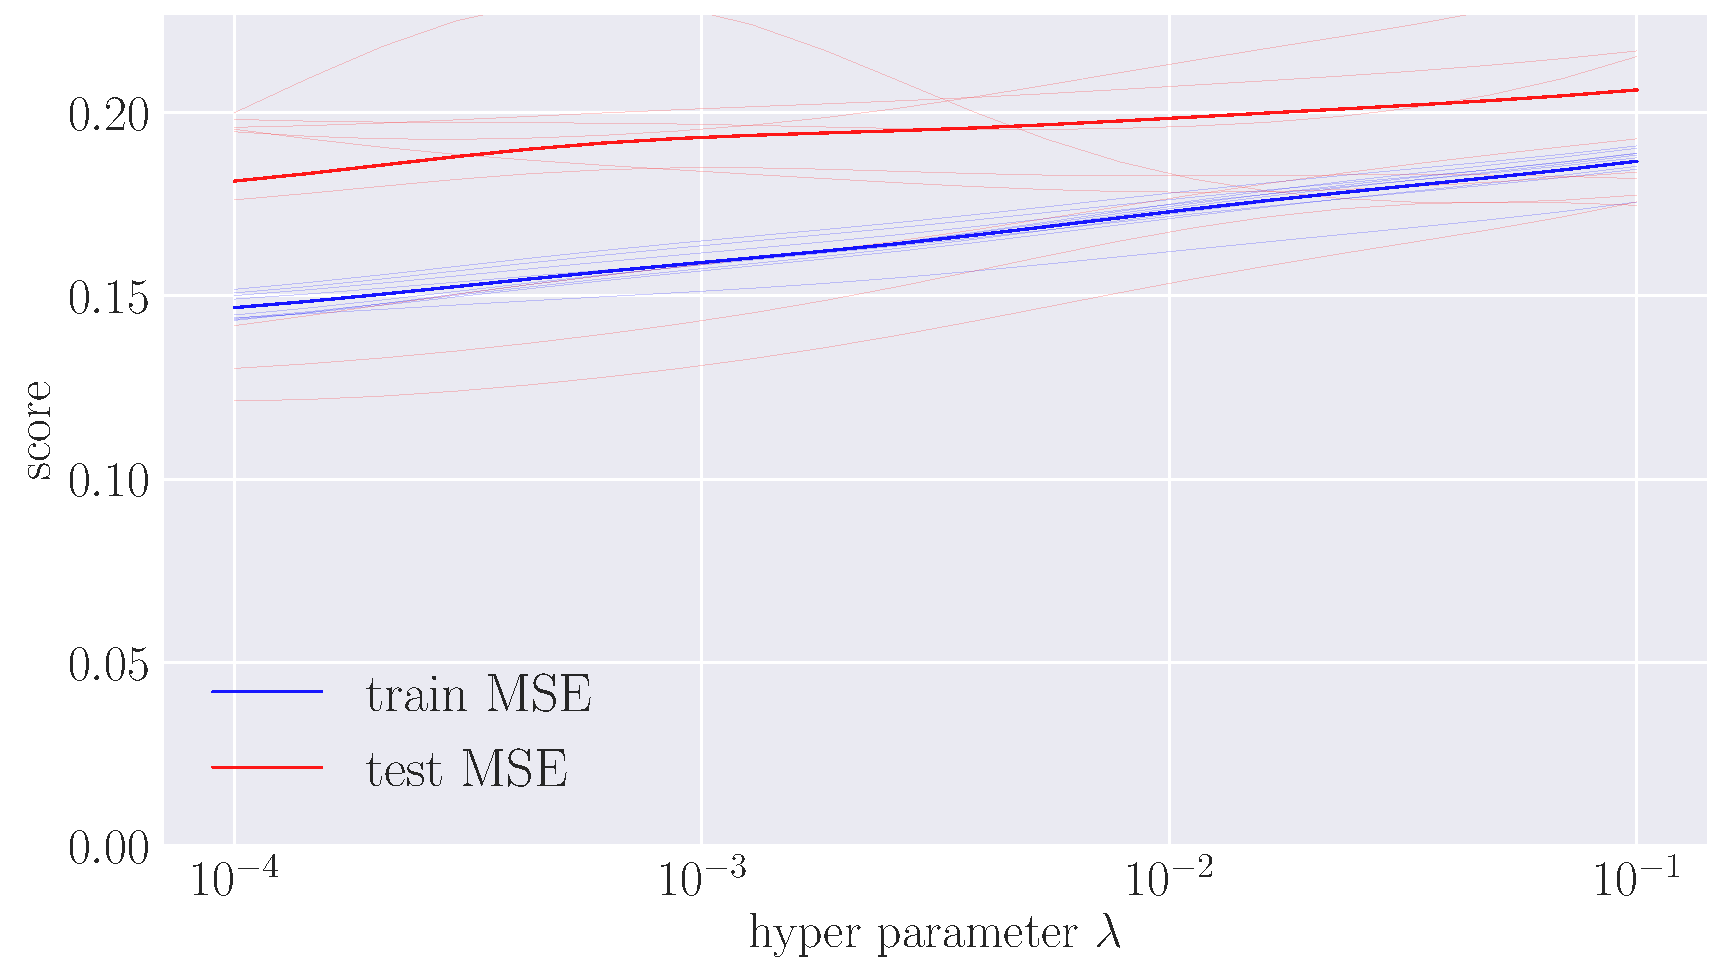
\includegraphics[width=\linewidth]{ptE_CV_Ridge.pdf}
            \caption{Cross-validation for Ridge regression.}
            \label{eq:cross-validation_ridge}
        \end{figure}

        \begin{figure}
            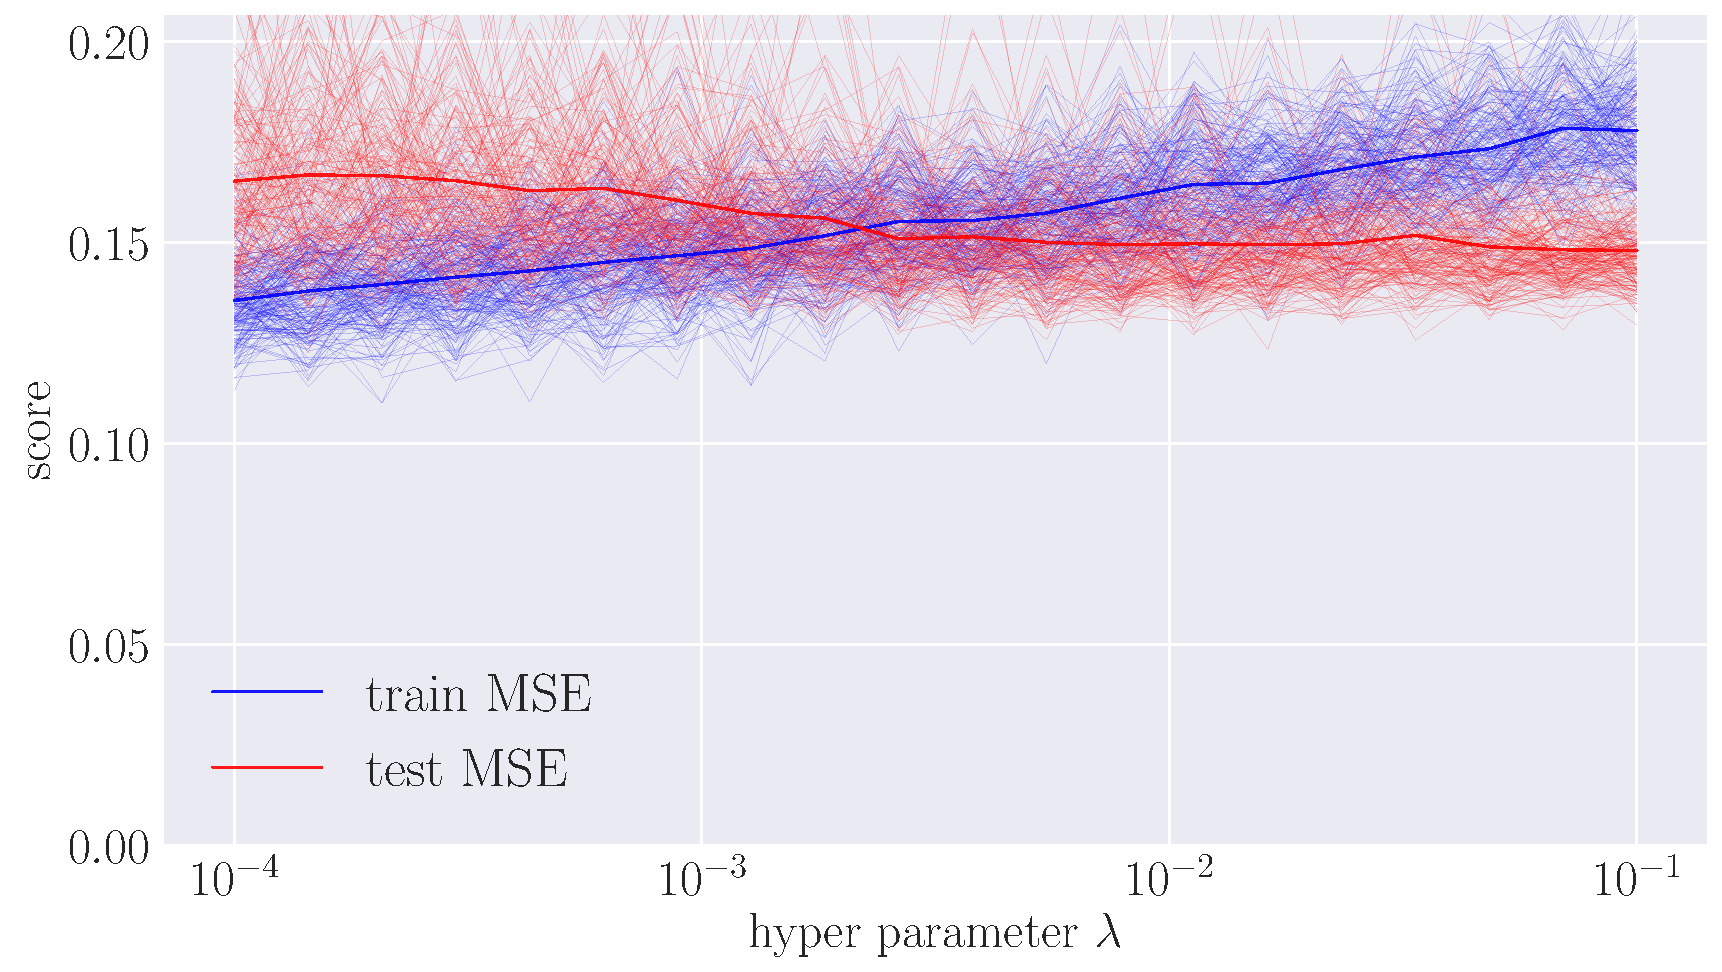
\includegraphics[width=\linewidth]{ptE_Hastie_Ridge.pdf}
            \caption{Model complexity for Ridge regression.}
            \label{eq:model_complexity_ridge}
        \end{figure}

        \begin{figure}
            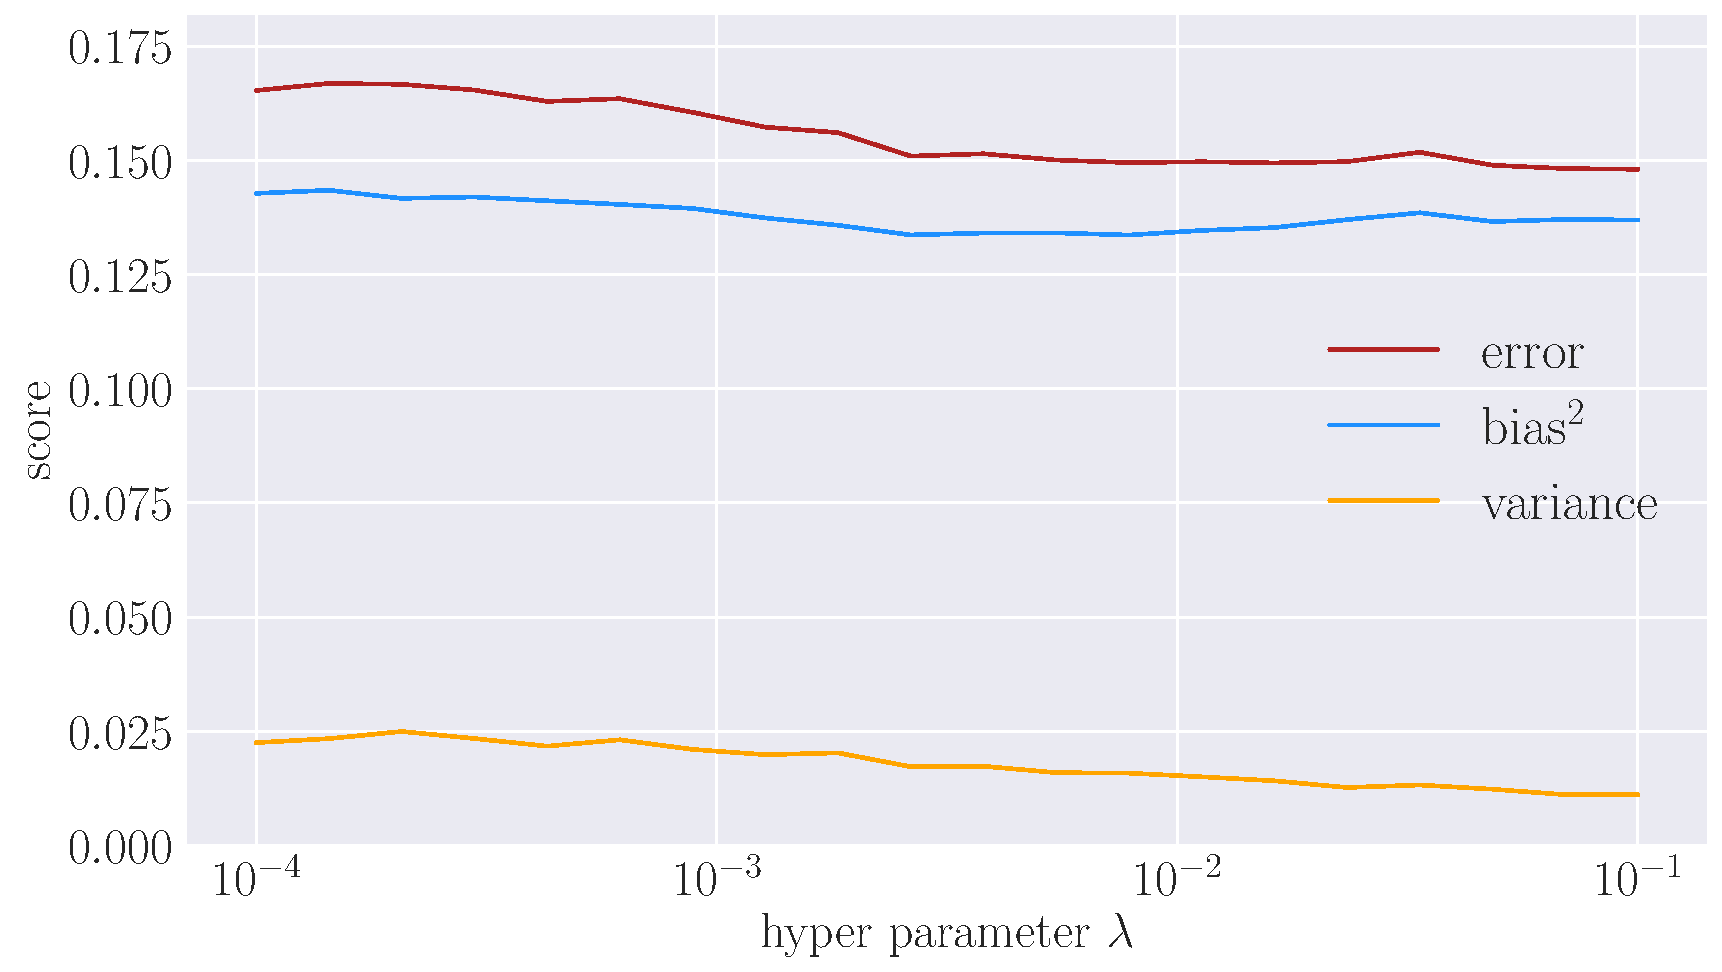
\includegraphics[width=\linewidth]{ptE_tradeoff_Ridge.pdf}
            \caption{Bias-variance for Ridge regression.}
            \label{eq:bias_variance_ridge}
        \end{figure}

        \subsubsection{Lasso}\label{sec:lassoanalysis}

    \subsection{Applying best fit model}\label{sec:applybestmodel}

    \subsection{Real terrain data}\label{sec:realdata}